\subsection{Aufbau}
Der Aufbau des Experiments ist in folgender Abbildung dargestellt:
\begin{figure}[h!]
  \centering
  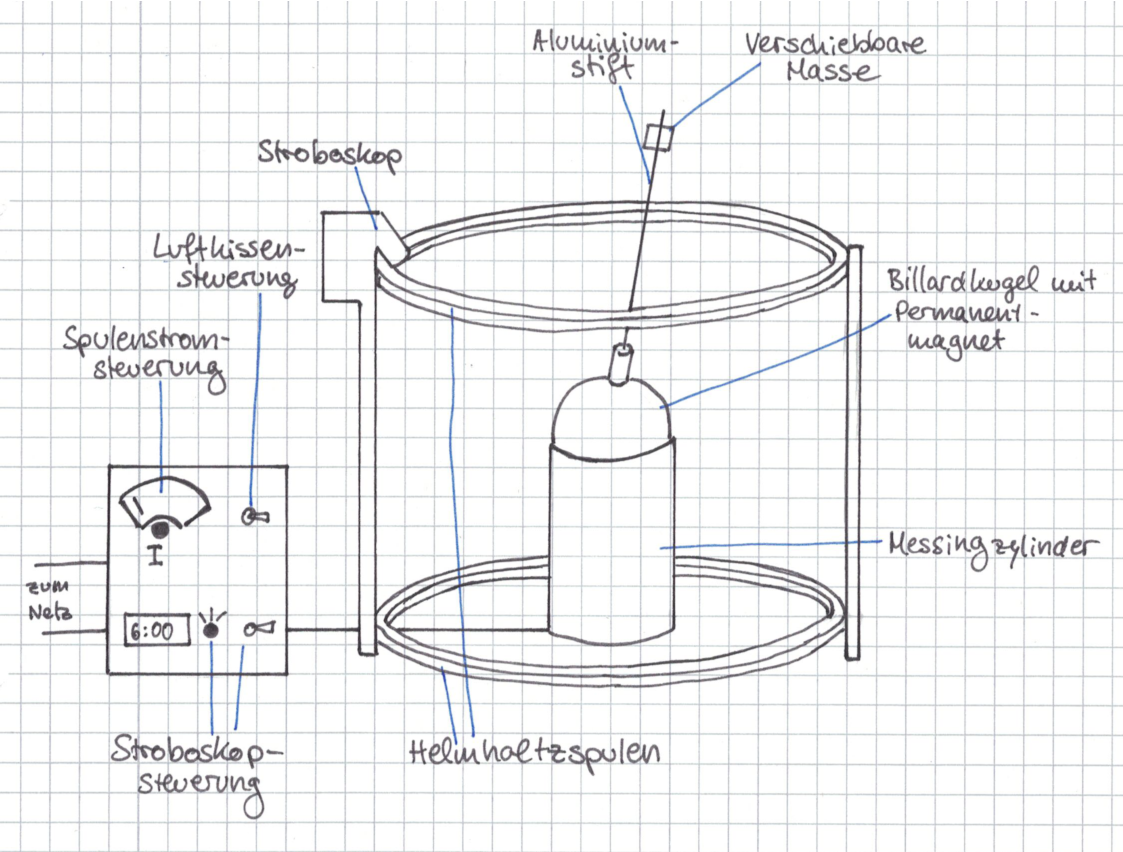
\includegraphics[width=\textwidth]{Aufbau.pdf}
  \caption{Schematischer Aufbau der Messapparatur}
  \label{aufbau}
\end{figure}
\\Ein Permanentmagnet ist in eine Kugel eingelassen, hier Billardkugel genannt.
Ein Messingzylinder steht in der Mitte eines Helmholtzspulenpaars mit den Abmessungen $N=195$, $d=\SI{0.138}{m}$ und $R=\SI{0.109}{m}$.
Die Billardkugel wird auf ein Luftkissen auf dem Messingzylinder gelegt.
Am Rand der oberen Helmholtzspule ist ein Stroboskoplicht angebracht.
An dem Steuergerät können die Magnetfeld-erzeugende Stromstärke an den Spulen und das Stroboskop eingestellt werden.
Außerdem wird das Luftkissen über das Steuergerät ein- und ausgeschaltet.

\subsection{Durchführung der Bestimmung des magnetischen Momentes unter Ausnutzung der Gravitation}
Für diese Methode wird eine verschiebbare Masse an einem dünnen Aluminiumstift in die Billardkugel gesteckt.
Die Masse wird als Punktmasse angesehen und die Masse des Aluminiumstiftes wird vernachlässigt.
Das Luftkissen wird eingeschaltet und die Richtung des Magnetfelds so eingestellt, dass es nach oben wirkt.
Der Radius der Masse vom Mittelpunkt der Billardkugel wird mithilfe einer Schieblehre festgelegt und die Billardkugel auf das Luftkissen gesetzt.
Dann wird der Spulenstrom so weit hochgedreht, bis die Kräfte in einem Gleichgewicht sind und die Billardkugel nicht mehr umkippt.
Der gesetzte Radius der Masse zum Mittelpunkt der Billardkugel und die Spulenstromstärke werden notiert.
Aus der Stromstärke wird das entsprechende Magnetfeld berechnet.
Die Messung wird für insgesamt 14 Radien durchgeführt.

\subsection{Durchführung der Bestimmung des magnetischen Momentes über die Schwingungsdauer des Magneten}
Bei dieser Methode wird zunächst das Luftkissen angestellt.
Die Richtung des Magnetfelds ist nach oben gehend.
Die Spulenstromstärke wird eingestellt und die Billardkugel wird auf dem Luftkissen vorsichtig ausgelenkt.
Die Schwingungsdauer von zehn Schwingungen wird gemesssen.
Daraus wird die Dauer einer Schwingung gemittelt.
Es werden die Spulenstromstärke und die gemittelte Schwingungsdauer notiert.
Die Messung wird mit 13 weiteren Stromstärken durchgeführt.

\subsection{Durchführung der Bestimmung des magnetischen Momentes über die Präzession der Billardkugel}
Es wird das Luftkissen eingeschaltet.
Das Stroboskoplicht wird auf eine Frequenz von 6Hz geregelt.
Anschließend wird die Billardkugel auf dem Luftkissen in Rotation versetzt und das Stroboskoplicht angestellt.
Sobald der weiße Punkt auf der Billardkugel als konstant, nicht mehr blinkend, wahrgenommen wird, wird die Billardkugel vorsichtig ausgelenkt und die Spulenstromstärke aufgedreht.
Die Umlaufdauer der Präzessionsbewegung wird gemessen und gemeinsam mit der Spulenstromstärke notiert.
Die Messung wird für die selbe Stromstärke drei mal wiederholt und die Umlaufzeiten gemittelt.
Die Messung wird für insgesamt zehn verschiedene Spulenstromstärken durchgeführt.
